\chapter{Pipeline Shell}
\label{ch:PipelineShell}

%\textbf{\Cref{issReq:update}}
%\textbf{\Cref{issReq:maintained}}


\tmp{Describe what the pipeline shell is and what it should do}

The \gls{ps} is a shell built around an ISS, that should control the ISS, gather the resulting state changes from the ISS, and output these at the correct time. The pipeline shell should also take in the asynchronous inputs, determine when and how these should be handled, control the ISS, and adapt the output accordingly. 

\section{Implementation strategy}

\begin{enumerate}
    \item Implement Spike integration by stepping spike when the core retires an instruction.
    \item This should pass all synchronous tests, but not asynchronous interrupt and debug tests
    \item Make test to pass interrupts to the RM and core
    \item Pass interrupts to spike in sync with RVFI from the core to develop correct interrupt handling in spike
    \item Pass interrupts to RM asynchronously. The directed test should fail since no pipeline shell is implemented
    \item Develop pipeline shell to correctly time interrupts. The directed test should pass
    \begin{enumerate}
        \item Model simple sequential pipeline that passes synchronous tests
        \item Handle interrupts correctly in situations where interrupts can be taken immediately
        \item Correctly model each of the signals in \sv{interrupt_allowed} to properly time interrupts in instances when they can not be taken immediately
        \item Correctly move the instructions through the pipeline so the signals in \sv{interrupt_allowed} are properly timed
    \end{enumerate}
\end{enumerate}

\section{Rquirements}

\begin{enumerate}

\item \textbf{RVFI from ISS.} \label{psReq:rvfi}
\par The pipeline shell should use \acrshort{rvfi} as the input interface from the ISS.

\item \textbf{The pipeline shell should be the only core-dependent component} \label{psReq:}
\par 

\item \textbf{} \label{psReq:}
\par 
\item \textbf{} \label{psReq:}
\par 
\item \textbf{} \label{psReq:}
\par 
\item \textbf{} \label{psReq:}
\par 
\end{enumerate}

\section{General architecture}

As discussed in \Cref{ch:design}, the pipeline shell should control the functional ISS, and correctly time the output state changes from the ISS. According to \Cref{psReq:rvfi}, the ISS should return the state changes as RVFI signals.


\subsection{Pipeline Shell Design}

\Cref{sec:pw_pipelineShellDesign} describes two possible pipeline shell designs; a \textit{stage-based pipeline simulation} modeled closely to an actual pipeline, and a \textit{cycle-based time wheel simulation}, similar to the approach by \textcite{chiangEfficientTwolayeredCycleaccurate2009}. 

The cycle-based approach stores the state changes into individual stages for each cycle, while the stage-based approach operates more closely to a normal pipeline.
\Cref{sec:pw_pipelineShellDesign} highlights some disadvantages of using a cycle-based approach, as the design makes some operations like flushing more complicated. 

When considering a pipeline shell that is compatible with formal verification, even more disadvantages with a cycle-based approach are uncovered. The cycle-based approach proposed by \textcite{chiangEfficientTwolayeredCycleaccurate2009} is written in SystemC. Since the \textit{time wheel} must have one stage for every cycle that an instruction is in the pipeline, the time wheel must have a dynamic size. This is problematic because dynamic arrays in SystemVerilog are not synthesizable\cite{mehtaIntroductionSystemVerilog2021}, and therefore not compatible with formal verification\cite{seligmanFormalVerificationEssential2015}.

Because of this, we choose to go with a stage-based pipeline shell. By doing so, we also have to be aware of the problem discussed in \Cref{sec:pw_pipelineShellDesign}, where bugs can be implemented the same way in both the reference model and core, and be undetected.

The architecture of the pipeline shell is shown in \Cref{fig:pipeline_shell}. \tmp{Explain figure}

\begin{figure}
    \centering
    \includegraphics[width=0.75\linewidth]{figures/Pipeline_shell.pdf}
    \caption{Architecture of pipeline shell}
    \label{fig:pipeline_shell}
\end{figure}

\subsection{Interaction with the ISS}

There are multiple choices regarding how to interact with the ISS. Some of these are discussed in \Cref{sec:pw_partition}
\tmp{When to call the ISS: -> IF}

\subsection{Compartementalizing core-specific functionality}

The pipeline shell should contain the core-specific timing implementation and be modifiable to different cores. To make it easy to configure for new cores, we should also compartmentalize the core-specific details of the pipeline shell so necessary modifications for a new core are kept to a minimum.


\subsection{General design choices}

\begin{itemize}
    \item Keep the pipeline shell as simple as possible. Let the ISS do as much work as possible
    \item Keep core specialized parts contained
\end{itemize}


\section{Dependency of core}
\label{sec:ps_dependency}

There are multiple options when deciding when instructions should move through the pipeline shell. We can separate these options into two categories: A \textit{retirement dependent approach}, where instructions are moved through the pipeline based on retirements from the core, and a \textit{core independent approach}, where the reference model is fully independent of the core and has to fully model the pipeline movement independent on what the core does. 

\subsection{Retirement dependent pipeline shell}

In a retirement-dependent pipeline shell, instructions are moved through the pipeline stages based on instruction retirements from the core. This is similar to a \textit{step-and-compare} approach from \Cref{sec:step-and-compare} where the ISS steps through an instruction when an instruction retires from the core. This allows the core and reference model to easily stay in sync without exactly mirroring the cycle-accurate execution of the core.


\subsection{Core independent pipeline shell}

In a core-independent pipeline shell, the execution would be fully independent of the core, and the movement of instructions through the pipeline would be completely contained in the pipeline shell. This complicates the pipeline shell because the pipeline shell has to mirror the exact execution of the core at every cycle. It must account for forwarding hazards and stalls, the exact cycle delay for \acrshort{lsu} operations, the exact cycle count of multi-cycle instructions, etc.

Instructions can be moved through the pipeline mirroring the functionality of the core, where every clock each stage reports if it is ready to receive new data, and if each stage has valid data ready, and uses this to move the data through the pipeline. Additionally, there are signals for pending interrupts, jumps, branches, exceptions, multi-cycle instructions in progress, etc. that must be considered. 

The CV32E40S user manual contains a table with the number of clock cycles for every multi-cycle instruction \cite{openhwgroupPipelineDetails2023}. If we do not rely on the retirement from the core, we must use this table to determine how long an instruction should take in each stage. This can be complicated as we need to have specific cases for every instruction, and some instruction types have different clock cycles for different situations.

%\tmp{40s security feature}

\subsection{comparison}

\begin{table}[htb]
\centering
\caption{Comparison of retirement and clock driven pipeline}
\label{tab:retirementvsclock}
\begin{tabularx}{\textwidth}{|p{15mm}|*{2}{>{\arraybackslash} X |}}
\hline
 & Advantages & Disadvantages \\
\hline
Retirement dependent
& \begin{itemize}
\item Simpler to model
\item Lower chance of implementing bugs from the core
\end{itemize}
& \begin{itemize}
\item Does not test if instructions retire after the right amount of cycles (Not that important?)
\item Add specific stall cases instead of movement cases
\item Will not be equal at every clock cycle
\item 
\end{itemize} \\
\hline
Core independent
& \begin{itemize}
\item Cycle-accurate equal to core
\item Can be used to verify that the core uses the correct amount of cycles for each instruction. 
\end{itemize}
& \begin{itemize}
\item Hard to implement. Essentially all timing-related implementations must be implemented in the core
\item We must calculate the cycle count for all instructions and edge cases.
\end{itemize} \\
\hline
\end{tabularx}
\end{table}

As discussed in \Cref{sec:des_retireOrClock}, we will only compare the state after each retirement, but cycle-accurate detail influences this as explained in \ref{}\tmp{TODO}.
Since we only compare the core and reference model at instruction retirements, it might be sufficient with a retirement-dependent pipeline shell. If this works, it would be easier to implement and less complicated. We would not need to model as much of the core-specific details. To avoid the possibility of implementing the same bugs that might be in the core, we want to avoid implementing detailed core-specific details as much as possible.

\textbf{Design choice:} We will focus on a retirement-dependent pipeline shell going forward to determine if this is sufficient. 



%\begin{enumerate}
%    \item Should the pipeline shell calculate the correct clock cycle for each instruction? Hard for division etc which is variable.
%    \item Can retirements be used and potential "bubbles" be calculated instead of all details 
%    \item What in the dependency graph can be wrong if we only move the pipeline on retirements?
%    \item - Can these occurrences be specifically handled, instead of accurately calculating all "instruction movements?"
%    \item How should stalls be calculated?
%    \item How should pipeline flushes be handled?
%    \item How should multi cycle instruction be handled?
%\end{enumerate}


\section{Datapath / Pipeline modules design}

This section will cover the design choices for the actual pipeline stages that the instructions should travel through. 

\subsection{Pipeline stages}

We want most of the timing details to happen in the controller module with our chosen architecture, leaving the pipeline modules fairly simple. This gives us the choice of making separate modules for each pipeline stage, or reusing the same module for all the stages. Although the pipeline stages should operate fairly similarly, there are some differences. For example, the IF stage must step the ISS and take in the RVFI from the ISS as an input. By making separate modules for each pipeline stage, we can specifically modify IF to call the step function, and take the RVFI result from the pipeline. If we instead use a generic stage module, we have to call the step function outside of the IF stage. 

Different cores can have different numbers of pipeline stages, so it should also be trivial to add or remove pipeline stages when configuring the pipeline shell for a new core. The pipeline shell could use a generate construct to change the number of pipeline stages. This would also lead to a differing number of inputs and outputs to the controller module, which should control each step. For this, an interface could be used with a configurable number of control signals for each pipeline stage. Alternatively, we can have different pipeline shell files for each core in separate directories that can be more specialized for the core. A parameterizable amount of pipeline stages could work for in-order pipelines, but this could get more complicated if we also consider out-of-order pipelines. This report will focus on in-order pipelines, but to possibly also allow out-of-order pipelines, we choose to go with the second option, where all the pipeline shell files are specific to a core.

\tmp{TODO: Use an interface with rvfi and control signals instead of individual signals.}

%\textbf{Design choice:} Use a generic pipeline stage module, or specific for each stage? \tmp{currently specific but not justified}
%
%Generic: easier to add more pipeline stages.
%
%Specific: Not all pipeline stages are equal.
%
%For the IF stage, we call the \sv{iss_step()}function to step spike. This can either be done inside of the if module with a specific stage module, or outside the module and passed in as a \sv{pipe_stage_t} input, that is used by the other stages to move data from the previous stage.
%
%\tmp{The core has a delay between the WB stage and the RVFI output, replicate this in the RM or use straight out of WB?}
%
%
%\tmp{General or specific pipeline stage modules? IF and WB are slightly different compared to the others.}

\subsection{pipeline stage register content}

\begin{itemize}
    \item RVFI from ISS: \textbf{\Cref{issReq:state}}
    \item Valid
\end{itemize}

To properly output the RVFI value when an instruction has moved through the pipeline, we need to know if the instruction in each pipeline stage is valid.
We therefore add a valid signal that is high when the instruction executed correctly in the ISS, and goes low before before the pipeline is filled up, when the pipeline is flushed, etc.

We combine these signals into a struct, so that potential future signals can easily be added.
\begin{systemverilog}
typedef struct packed {
    st_rvfi rvfi;
    logic valid;
} pipe_stage_t; 
\end{systemverilog}


Since we use instruction retirements from the core to move through the pipeline stages, we also need to use this to output RVFI. To make sure each instruction is only marked as valid for one cycle when outputting rvfi, we need to combine the valid signal from the core, with the valid signal from the pipeline shell. This allows the RVFI output to be in sync with the core, while also only outputting RVFI when the instruction in the pipeline shell is actually valid.

The WB stage therefore looks like this.
\begin{systemverilog}
always_ff @(posedge clk) begin
    if (flush_i) begin
        pipe_o.rvfi <= '0;
        pipe_o.valid <= 1'b0;
    end else if(step) begin
        pipe_o.rvfi <= pipe_i.rvfi;
        pipe_o.valid <= pipe_i.valid;
    end
    else begin
        pipe_o.rvfi <= pipe_o.rvfi;
        pipe_o.valid <= 1'b0; //Only output valid at first valid clock cycle
    end
end
\end{systemverilog}

\subsection{Register in the WB stage}

As shown in \Cref{fig:cv32e40s-block}, the CV32E40S core the pipeline has 3 registers between the 4 pipeline stages: \sv{IF_ID},\sv{ID_EX}, and \sv{EX_WB}. What is not shown in the figure is that the RVFI output, which should be valid when an instruction is retired, is actually delayed one cycle from when the instruction reaches the WB stage. To simulate this behaviour in our pipeline shell, we also add a register after the WB stage, giving us the pipeline in \Cref{fig:pipeline_shell}

\section{Controller module design}

The controller is the module that actually controls the movement of the pipeline stages, and is the part of the reference module that contains the most core-specifics.

\subsection{Requirements}

\begin{enumerate}
    \item Determine when to step the ISS and pipeline stages based on retirements from the core
    \item Control flushing of the pipeline stages
    \item Control if an interrupt can be taken and corresponding flushing
    \item Fill up pipeline after flushing
    \item Control the ISS state revertion?
    \item Handle debug requests
    \item Handle \acrshort{nmi}s
\end{enumerate}

\subsubsection{Input signals}
\begin{itemize}
    \item \sv{clk}
    \item \sv{rst}
    \item \sv{valid} (Retirement from the core)
    \item \sv{irq_i} 
    \item \sv{if_id_pipe_i}
    \item \sv{id_ex_pipe_i}
    \item \sv{ex_wb_pipe_i} 
    \item \sv{wb_pipe_i}
    \item \sv{interrupt_allowed_i} interrupt allowed from the core
    \item \sv{mstatus.mie} from the ISS
\end{itemize}

\subsubsection{Output signals}
\begin{itemize}
    \item \sv{\{if,id,ex,wb\}_step_o}
    \item \sv{\{if,id,ex,wb\}_flush_o}
    \item \sv{interrupt_allowed_o}
\end{itemize}


\subsubsection{Tasks}

\begin{itemize}
    \item Flush pipeline when an interrupt is taken
    \item Refill the pipeline after a flush
    \item Step the pipeline when the Core retires an instruction
    \item Control the interrupt allowed signal. It should go high when mie is high in WB and the interrupt is allowed, and should go low when an interrupt is taken, even before mie goes low in WB 
    \item Call \sv{iss_intr()} every clock with 
\end{itemize}


\tmp{FSM?}



\subsection{interrupts}

\section{Instruction stepping}

\subsection{instruction stepping}

We will use the word \textit{\gls{step}} to mean when the ISS executes one instruction and when an instruction moves from one pipeline stage to another. When implementing a retirement-dependent pipeline shell, we want to step the ISS and pipeline stages when the core retires an instruction.

In a normal pipeline, the movement of instructions in the pipeline is controlled by a \sv{ready} and a \sv{valid} signal in each pipeline stage. When both the previous stage has \sv{valid} data, and the next stage is \sv{ready} to receive new data, the instruction data is moved into the next pipeline register.

Since we use a step function and a simplified pipeline, we can instead use a \sv{step} signal to step the pipeline. The same step signal can be used to step the ISS and step the pipeline to ensure this happens in sync.

To step the ISS, we need a function that will step one instruction when called. This gives us \textbf{\Cref{issReq:step}}. Since we use a retirement-dependent approach, we will call this step function when the core retires an instruction, and the \sv{rvfi_valid} signal is high. 

\subsection{halting}

In a normal pipeline, every stage can be halted, where the pipeline stage will not be valid or ready, meaning it will not be updated with a previous instruction or output its value to a new stage. Since we use a \sv{step} signal to signal when an instruction should step into the next pipeline stage or not, this implicitly supports halts without needing a separate halt signal. 

\subsection{Filling the pipeline}

At the very beginning of a simulation and after the pipeline is flushed, it contains multiple empty stages. If we wait for the first retirement from the core before executing any instructions in the reference model, it would be delayed behind the core since it takes multiple steps to fill up the pipeline and output instructions. 

Because of this, we want to fill up the pipeline when it is not full so that the next retirement from the core also triggers a retirement from the reference model.

To implement this functionality, we use a \sv{pipe_count} counter that starts at 0 at the beginning and is reset to 0 during a full pipeline flush. This counts up to the number of pipeline stages every time a step is done. This keeps track of how many instructions are in the pipeline. When the counter is lower than the number of pipeline stages, we set \sv{step} high so the pipeline can fill up. When the pipeline is filled, the \sv{step} signal is controlled by the \sv{rvfi_valid} signal from the core. This is shown in \Cref{lst:pipe_count}.

\begin{systemverilog}[label={lst:pipe_count}, caption={Systemverilog code for filling the pipeline at the start and after a flush.}]

assign pipeline_full = pipe_count >= (PIPELINE_DEPTH - 1);

// Count the amount of filled pipeline stages at the start or after a flush 
always_ff @(posedge clk) begin
    if (rst_n == 1'b0 || flush_pipeline)begin 
        pipe_count <= 0;
    end else if (!pipeline_full) begin
        pipe_count <= pipe_count + 1;
    end else begin
        pipe_count <= pipe_count;
    end
end
// step the pipeline until the first stages are filled up to be in sync with the core
always_comb begin
    if (rst_n == 1'b0) begin
        step <= 1'b0;
    end else if (!pipeline_full) begin
        step <= 1'b1;
    end
    else if (valid) begin
        step <= 1'b1;
    end
    else begin
        step <= 1'b0;
    end
end
\end{systemverilog}



\section{Timing Side effects}
\label{sec:side-effects}

\subsection{Side effects influencing interrupt timing}

Some side effects affect the timing of interrupts. These are \rv{mstatus.mie} and \rv{mie}. To properly time interrupts, we want to apply the changes in these CSRs when they leave the WB stage in the pipeline shell, instead of when the instruction steps in the IF stage.


Since we step the instruction in the ISS in the IF stage, there are some cycles before the instruction is retired from the reference model, because it travels through the pipeline stages. If we use the CSR registers local to the ISS, these might not be the same as if they were updated in the WB stage.

\begin{figure}
    \centering
    \includegraphics[width=1\linewidth]{figures/mret_example_fail.pdf}
    \caption{Example showing the mismatch of execution between the core and reference model when an interrupt is taken directly after another interrupt.}
    \label{fig:mret_example_fail}
\end{figure}


This can be highlighted with the example in \Cref{fig:mret_example_fail}. This shows the pipeline content of the core and reference model, aswell as the \rv{mie} bit in the \rv{mstatus} CSR. In the example, the reference model uses the CSR stored in the ISS to determine if interrupts are enabled or disabled.

The example shows an interrupt being applied while another interrupt handler is running (orange instructions). As explained in \Cref{sec:bg_interrupts}, when an interrupt is taken, and the interrupt handler starts running. This disables the \rv{mstatus.mie} bit. At the end of the interrupt handler, the \rv{mret} instruction runs to return to normal execution, and enables \rv{mstatus.mie} again. 


The example shows that when the \rv{mret} instruction runs in the ISS, \rv{mstatue.mie} is immediately enabled. If another interrupt is enabled at this point, the ISS would then take the next interrupt directly after the mret, instead of returning to the normal execution flow (green instructions) like the core does. We see that this causes the instructions with PC \rv{0001714E, 00017152, and 00017156} to not be retired from the core before the interrupt is taken.


\subsection{External CSR}

To avoid this mistake, we must consider the timing of the CSR writes through the pipeline.

One way to do this is to add an external CSR to the pipeline shell. This can hold the CSRs that affect the interrupt timing and can be updated based on the pipeline content. When calling the interrupt function in the ISS, we can add the updated contents of the external CSR to enable interrupts only when the CSR changes have properly propagated to the external CSR.

CSR changes can be output with RVFI. Since the RVFI output of the ISS already travels through the pipeline, we can use this to update the external CSR when the changes reach the WB stage.


\Cref{fig:mret_example} shows the same example as above, but the value from the external CSR is considered before taking an interrupt. The example shows both the CSR from the ISS and the external CSR.

\begin{figure}
    \centering
    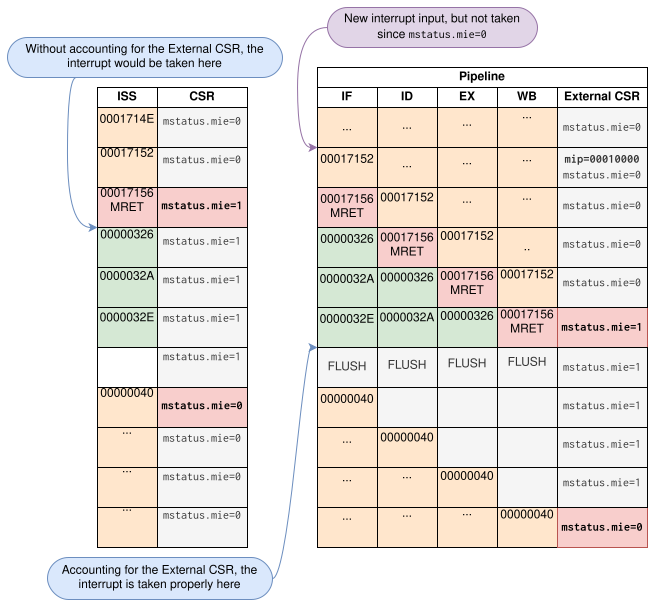
\includegraphics[width=1\linewidth]{figures/mret_example.pdf}
    \caption{Example showing how the timing of CSRs can influence interrupt timing.}
    \label{fig:mret_example}
\end{figure}

We see that in the ISS, the interrupt is not immediately taken after the \rv{mret} instruction, but instead taken when the external CSR changes to \rv{mstatus.mie=1}.

It can be beneficial to also use the CSR from the ISS, because although we want to delay the enabling of the interrupt, we want interrupts to be immediately disabled when an interrupt is taken. From the figure, we se the external CSR also delays the disabling of \rv{mstatus.mie}. If we only used the external CSR, new interrupts could be taken after another interrupt is taken. Because of this it is beneficial to use both the internal and external CSR.

The same problem can occur immediately following a write to the \rv{mie} CSR that enables a previously disabled \rv{irq}. It can also be solved the same way, by storing \rv{mie} in the external CSR.




\section{Interrupt}
\label{sec:ps_interrupt}

\subsection{Interrupt timing in the core}

When taking an interrupt there are multiple considerations. \Cref{fig:interrupt_timing} shows a simplified diagram of what affects the timing of an interrupt in the CV32E40S core, divided into clock cycles. We see that the interrupt is applied in cycle N. The next cycle, the interrupt is clocked into \sv{irq_q}. In cycle N+1, it is decided wether the interrupt will be taken or not, given the result of the \sv{pending_interrupt} and \sv{interrupt_allowed} signals. \sv{pending_interrupt} depends on the interrupt, wether the specific interrupt is enabled in \rv{mie}, and wether all interrupts are allowed with \rv{mstatus.mie}. \sv{interrupt_allowed} depends on the state of the pipeline, and determines if the pipeline can safely be flushed. If the interrupt can be taken, the PC is changed to the interrupt handler. In cycle N+2 the pipeline is flushed and interrupt handler instruction is prefetched and clocked into the IF stage register in cycle N+3. It propagates through the pipeline and is retired and output to RVFI at cycle N+6.

\begin{figure}
    \centering
    \includegraphics[width=1\linewidth]{figures/interrupt_handeling_timing.pdf}
    \caption{Diagram showing the components that effect the timing of taking an interrupt.}
    \label{fig:interrupt_timing}
\end{figure}


\subsection{Taking interrupts in the reference model}

The decision of wether to take the interrupt can either be done in the ISS, or in the controller of the pipeline shell. If the pipeline shell should decide wether an interrupt should be taken all the information that influences this needs to be exported from the ISS. This includes the \rv{mie} and \rv{mstatus} CSRs, the privilege level, the debug mode, etc. If we want to evaluate this in the ISS, we need to ensure that the ISS has access to the correctly timed CSRs from the external CSR. 


\subsubsection{Decision in pipeline shell or ISS}

\tmp{TODO: Move decision to PS or not?}

Compared to the core, the pipeline shell of the reference model does not have access to all the CSRs without exporting them from the \acrshort{iss}. In order to determine if an incoming interrupt will actually be taken, we need to know the values of \sv{mie}, \sv{mstatus.mie} and the privilege level. As these are all kept inside the \acrshort{iss}, we either have to export these from the ISS, or determine if the interrupt will be taken inside the ISS. 

This check can be combined with the \sv{iss_intr(irq)} used to signal a new interrupt to the ISS. The function can return true if the signaled interrupt will be taken, and false if any of the CRSs will cause the interrupt to not be taken. The \sv{interrupt_allowed} signal does not depend on the ISS, but rather the content of the pipeline, so the ISS will only calculate the \sv{pending_interrupt} signal. Because of this, the \sv{iss_intr(irq)} function should only be called when the \sv{interrupt_allowed} signal is high. If it is low, the processor execution should continue as usual until \sv{interrupt_allowed} goes high.

In the core, the \sv{mip} bits are set every clock cycle independently of the value of \sv{interrupt_allowed} or if interrupts are enabled in the \acrshort{csr}s \cite{}.

\textbf{Design choice:} Call \sv{iss_intr()} every retirement, when mip changes, only when interrupts are allowed, or only when interrupts are enabled? -> Every clock, but add checks inside to check if the interrupt is new


We can divide interrupt taking into two decisions, when to take an interrupt, and which interrupt to take.

\subsubsection{Which interrupt to take}

To decide which interrupt to take, we can either determine this in the pipeline shell, or we can let the ISS decide itself. This approach simplifies the interface to the ISS, since we can inject the whole \rv{irq} register into the ISS as is, to be set in the \rv{mip} register. By accurately setting the \rv{mip} bits, the ISS should be able to determine which interrupt to take.

This is not actually the case. The RISC-V specification only specifies the correct order of the standard interrupts specified in bit 15:0 in \rv{mip}, but not for the custom interrupt bits at bit 16 and above \cite{watermanRISCVInstructionSet2021}. If the ISS should decide the order of interrupts, some platform or core-specific interrupt handling information must be implemented in the ISS.

On the other hand, if we determine the interrupt ordering in the pipeline shell, it causes some problems with the communication with the ISS. Instead of injecting the bits to be set in \rv{mip} and let the ISS operate close to its original execution, larger modifications to interrupt handling is required. If we want to tell the ISS which interrupt to take, the ISS must be modified to take the input interrupt instead of analyzing \rv{mip} instead. One approach of informing the ISS of the interrupt is to only set one \rv{mip} bit at a time, so the ISS has no choice. This can work, but causes a mismatch between the \rv{mip} register of the core and the reference model. Another way would be to override the ISS interrupt-taking functionality so that it takes a given interrupt.
Neither of the approaches above are optimal, so we choose to let the ISS decide which interrupt to take, giving us \textbf{\Cref{issReq:interruptOrdering}}



\subsubsection{Interrupt allowed}

\tmp{TODO}

\subsubsection{interrupt enabled}

\tmp{TODO}

\subsection{inform ISS of interrupt}

To inform the ISS of interrupts, we can either use a separate \sv{iss_intr()} function or also use the \sv{iss_step()} function to inform the ISS of interrupts.
Since the step function only runs when the core retires an instructions, and we may want to inform the ISS of interrupts independently of retirements, we choose to use a separate interrupts function. This gives us \textbf{\Cref{issReq:interrupt}}.

We must decide when the \sv{iss_intr} function should be called and when the \rv{mip} bits should be updated. This can be done every clock cycle, whenever \sv{irq_q} changes, or only when interrupts are allowed.


One challenge is to keep the \rv{mip} bits correct while interrupts are not enabled. If the \sv{irq} bits change while interrupts are not allowed, subsequent reads of the \rv{mip} CSR would be incorrect if the \rv{mip} bits are not written to when interrupts are not allowed.


To overcome this, the \sv{iss_intr()} function can be expanded to take \sv{irq_q} and \sv{interrupt_allowed} as inputs. This way, it can be called every clock cycle or whenever \sv{irq_q} changes. If \sv{interrupt_allowed == 0}, the \rv{mip} will be set, but the interrupt should not be taken. This implementation requires that the ISS can enable or disable interrupts, independently of the \rv{mip} bits and other CSRs, and that this can be controlled by the \sv{iss_intr()} function, giving us \Cref{issReq:mip}. 

One disadvantage of this approach is that it leads to many more DPI function calls to the ISS, which can decrease performance.


%To signal to the ISS when an interrupt should be taken, one way is to use the \rv{mip} bits to signal when it should be taken, and set these bits to 0 when the interrupt can not be take. This is problematic because situations can occur where the \rv{irq} bits change while interrupts are not allowed. This would lead to a mismatch between the \rv{mip} bits of the core and reference model. This could mostly go unnoticed, but be problematic if a CSR read is done on the \rv{mip} bits.  





%In spike this functionality is not possible. If \sv{mip} is set, and the interrupt is enabled through the CSRs, the interrupt will be taken the next time spike steps. It is therefore not possible to disable an interrupt with \sv{interrupt_allowed} while keeping all the CSRs identical to the core. To implement the \sv{interrupt_allowed} functionality, we must either only set the \sv{mip} bits when \sv{interrupt_allowed == 1}, disable the interrupt via a CSR like \sv{mstatus.mie}, or internally modify spike to implement an additional check on a new \sv{interrupt_allowed} variable before taking an interrupt, for example modifying \ccode{void processor_t::take_interrupt(reg_t pending_interrupts)} from \file{processor.cc} \cite{SpikeRISCVISA2023}. 



\subsection{Interupt taking}

To signal to the pipeline when an interrupt is taken, and the pipeline needs to be flushed, we can either use the return of \sv{iss_intr()} that says when the interrupt should be taken or use the RVFI output from the ISS. The RVFI is only output when the core retires an instruction, but there can be some time between when the interrupt is applied and when the core retires an instruction. The \sv{interrupt_taken} signal from \sv{iss_intr()} signals when the interrupt can be taken the clock after the interrupt is signaled, more closely resembling the core functionality. 







%\section{Taking an interrupt}
%
%\tmp{Use ISS to determine if it can be taken?}
%
% In the core, an interrupt is taken if both \sv{pending_interrupt} and \sv{interrupt_allowed} is true. \sv{interrupt_allowed} is explained in \Cref{sec:interrupttiming}. \sv{pending_interrupt} is high if an interrupt is set on \sv{irq_q} and the same bit is enabled in the \sv{mie} \acrshort{csr}. Additionally, the \sv{mstatus.mie} global interrupt enable \acrshort{csr} must be set, and the privilege level muse be below 
%
%By expanding the signals responsible for \sv{pending interrupt}, we get the expression in \Cref{lst:pending_interrupt}
%
%\begin{systemverilog}[label={lst:pending_interrupt}, caption={Signal requirements for \sv{pending_interrupt}}]
%    pending_interrupt = 
%    irq_req_ctrl_o = (|irq_local_qual) && global_irq_enable = 
%    (|irq_local_qual) && (mstatis_i.mie || (priv_lvl_i < PRIV_LVL_M) = 
%    (|(irq_q & mie_i)) && (mstatis_i.mie || (priv_lvl_i < PRIV_LVL_M)
%\end{systemverilog}
%
%When \sv{pending_interrupt} is high, we know that the interrupt on \sv{irq_q} will actually be taken if \sv{interrupt_allowed} also is high. 
%
%
%\subsubsection{Scenario: Set mip while \sv{interrupt_allowed = 1} and interrupt enabled.}
%
%Interrupt should be taken immediately.
%
%\subsubsection{Scenario: Set mip  while \sv{interrupt_allowed = 0}, interrupt enabled. Then set \sv{interrupt_allowed = 1}}
%
%Interrupt should be taken when \sv{interrupt_allowed} goes to 1. mip should remain set while \sv{interrupt_allowed} is 0
%
%\subsubsection{Scenario: Set mip  while \sv{interrupt_allowed = 1} and mie disabled, then later enable mie }
%
%\subsubsection{Scenario: Set mip  while \sv{interrupt_allowed = 0} and mie disabled, then later enabled enable mie, and set \sv{interrupt_allowed = 1}}
%
%
%
%\subsubsection{requirements}
%
%\sv{mip} should remain set or not while \sv{irq_q}
%In the core \sv{mip} directly follows \sv{irq_q}, independently of the other signals. 
%
%
%%In order to minimize modifications to the internal Spike code, and minimize the effect on other parts of the code, we choose to only set the \sv{mip} bits only when \sv{interrupt_allowed == 1}. 
%
%%This check can either be done in the \sv{iss_intr()} function, or before calling the function. To support the possibility changing to a solution where \sv{mip} is set independently of \sv{interrupt_allowed} like above, we implement the \sv{interrupt_allowed} check inside \sv{iss_intr()} to allow the rest of the code to be unchanged in both implementations.
%
%
%Regarding when to call the \sv{iss_intr()} function, the simplest implementation might be to call it at every positive clock edge. This avoids extra checks outside \sv{iss_intr()} to determine when it can and should be called, but instead keeps these check inside the function, dependent on implementation. 
%

\section{Flushing}

\tmp{Must the pipeline be flushed on branches or jumps?}

\tmp{If the ISS reports a jump or branch we can flush the pipeline.}

When the interrupt is taken, the remaining instructions in the pipeline must be \glsdisp{flush}{flushed}. This requires that the instructions in the pipeline should be set to 0, and the \sv{valid} signal be set to \sv{0}. This can be done by adding signals \sv{if_flush, id_flush, ex_flush}, and \sv{wb_flush} to each pipeline stage to flush each stage.

Since we only take interrupts when the pipeline can safely be flushed, we can directly use the \sv{interrupt_taken} signal to flush all the pipeline stages, as shown below.

\begin{systemverilog}
    assign flush_pipeline = interrupt_taken || debug_taken_q;

    always_comb begin
        if_flush_o <= flush_pipeline;
        id_flush_o <= flush_pipeline;
        ex_flush_o <= flush_pipeline;
        wb_flush_o <= flush_pipeline;
    end
\end{systemverilog}

\section{State Rollback}

\tmp{Why}
In a normal pipeline, where the state changes are applied in the WB stage, flushing each pipeline stage is sufficient to discard the effects of the instruction \cite[Ch. 4]{pattersonComputerOrganizationDesign2021}.

This is not necessarily the case for our pipeline implementation. Since the ISS executes the whole instruction before inputting the results into the IF stage, all the instruction's state changes are already written back inside the ISS. Since the changes have already been applied, flushing the pipeline does not discard them. To also discard these changes in the ISS, we need a way to revert the state of the ISS to a previous state.

This is one of the major disadvantages of calling the ISS in the IF stage compared to calling the ISS in the WB stage.


\tmp{What} 

This is in some ways comparable to the rollback approach used by some lock-step processors \cite{marquesLockVHeterogeneousFault2021, liDuckCoreFaultTolerantProcessor2021, nikiemaDesignLowComplexity2023} to \textit{rollback} the processor context of two synced cores if they diverge. \textcite{marquesLockVHeterogeneousFault2021} saves the state of the processor at various \glspl{checkpoint} along the execution, and if a fault is found, the state is reverted to the previous valid checkpoint.

We can use a similar approach, where we store the state of the ISS as checkpoints we can revert back to. Since an interrupt and flush can happen at any instruction, we should have a checkpoint between every instruction.

\tmp{What state elements need to be reverted}


\tmp{Store states in PS or ISS}

\tmp{How many states to revert}

\tmp{When to revert}





\section{State revertion}
\tmp{Rollback instead?}

%This is enough for a traditional pipeline where the instructions are committed in the last stage, but in our pipeline shell it gets more complicated because the instructions in the pipeline shell have already been fully executed in the ISS, and side effects have been applied. This is fine for normal execution, but requires that the ISS should be reverted to the state before the flushed instructions were executed.


\subsubsection{Experiment (Commit 0c2bc90c)}

\begin{clisting}
int customTest() {
    uint8_t interrupt = 16;
    
    printf("Division Test \n");

    active_test = 0;

    mstatus_mie_enable();

    //Enable all interrupts
    volatile uint32_t mie = (uint32_t) -1;
    __asm__ volatile("csrw mie, %0" : : "r" (mie));

    uint32_t a = 0x12341234;
    uint32_t b = 0x00004567;
    uint32_t result;

    __asm__ volatile("divu %0, %1, %2\n\t" : "=r" (result) : "r" (a), "r" (b));

    //Time interrupt in the middle of the division instruction
    mm_ram_assert_irq(0x1 << 16, 55);
    __asm__ volatile("divu %0, %1, %2\n\t" : "=r" (result) : "r" (a), "r" (b));
    __asm__ volatile("divu %0, %1, %2\n\t" : "=r" (result) : "r" (a), "r" (b));
    __asm__ volatile("divu %0, %1, %2\n\t" : "=r" (result) : "r" (a), "r" (b));

    mstatus_mie_disable();

    mie_disable(interrupt);

    return EXIT_SUCCESS;
}
\end{clisting}

The test applies an interrupt in the middle of an \rv{divu} instruction. During the instruction, \sv{interrupt_allowed} is stable high, so the interrupt should be taken immediately, aborting the current instruction.

Running the division test in \sv{custom_test()} in \file{custom_interrupt_test.c} 
The test is run with an implementation of flushing of pipeline stages, but not the discussed reversion of the spike states. 
When applying an interrupt in the middle of a long division operation, the interrupts are taken at the same retirement in the core and RM.

The problem arises in the interrupt handler and when returning after the interrupt handling as shown in \Cref{lst:divtest_error}.
In the core, instruction \sv{0000135c} was the last to finish, while in spike \sv{00001360} and \sv{00001364} were fully executed before being placed in the pipeline. The test fails first in the interrupt handler because the registers differ between the core and the RM because the RM wrote to registers that were not written to in the core. When returning from the trap handler, spike has stored another PC to \sv{mepc}, since it executed more instructions before being interrupted. This causes the execution to continue 2 instruction ahead of the core after returning from the interrupt handler. 


\begin{terminal}[caption={Errors from division test.}, label={lst:divtest_error}]
UVM_ERROR @ 13518.300 ns : uvmt_cv32e40s_reference_model_wrap.sv(48) reporter [Step-and-Compare] rd1_wdata core=0x12341234 and rm=0x00004325 PC=0x000008b8
# UVM_ERROR @ 13677.300 ns : uvmt_cv32e40s_reference_model_wrap.sv(48) reporter [Step-and-Compare] rd1_addr core=0x0000000d and rm=0x00000001 PC=0x00001360
# UVM_ERROR @ 13677.300 ns : uvmt_cv32e40s_reference_model_wrap.sv(48) reporter [Step-and-Compare] rd1_wdata core=0x00000007 and rm=0x00000368 PC=0x00001360
# UVM_ERROR @ 13677.300 ns : uvmt_cv32e40s_reference_model_wrap.sv(73) reporter [RVFI_PC] rvfi_rm.pc_rdata=1368 rvfi_core.pc_rdata=1360
# UVM_ERROR @ 13677.300 ns : uvmt_cv32e40s_reference_model_wrap.sv(77) reporter [RVFI_INSN] rvfi_rm.insn=fffff097 rvfi_core.insn=2e7d6b3
\end{terminal}


\begin{figure}[htb]
\centering
\input{figures/interrupt_revert_tikz}
\caption{\tmp{TODO: fix figure}Illustrate state reversion with ISS content and pipeline content.}
\label{fig:interrupt_revert_addi}
\end{figure}

\begin{figure}[htb]
\centering
\begin{ganttchart}[
		x unit=1.4cm,
		y unit chart=0.7cm,
		canvas/.style={draw=none,fill=none}, % remove canvas borders, etc
		vgrid={*{2}{draw=black!8}},           % vertical gray lines every unit
		inline,                              % draw bars inline
		group/.style={draw=none,fill=none},  % remove group borders, etc
		bar top shift=0.1,                   % give bar 10% padding top/bottom
		bar height=0.8,                      % bar size 80% of vertical space
		y unit title=0.5cm,                  % crop titles a little smaller
		title/.style={draw=none,fill=none},  % remove title borders, etc
		include title in canvas=false        % no vertical grid in title
	]{-2}{4}

    %\gantttitlelist{Cycle,IF,ID,EX,WB}{1}

	\gantttitle{Cycle}{-1}
	\gantttitle{ISS}{3}
 
	\gantttitle{}{1}
	\gantttitle{IF}{-1}
	\gantttitle{ID}{3}
	\gantttitle{EX}{-1}
	\gantttitle{WB}{3} \\

	\ganttgroup[inline=false]{1}{0}{4}
	\ganttbar[bar/.style={draw=black!80,fill=orange!40},name=iss0 ]{1}{-2}{-2}
	\ganttbar[bar/.style={draw=black!80,fill=orange!40}  ]{1}{0}{0}\\
 
	\ganttgroup[inline=false]{2}{0}{4}
	\ganttbar[bar/.style={draw=black!80,fill=yellow!40}, name=iss1  ]{2}{-2}{-2}
	\ganttbar[bar/.style={draw=black!80,fill=yellow!40}  ]{2}{0}{0}
	\ganttbar[bar/.style={draw=black!80,fill=orange!40}  ]{1}{1}{1}\\
 
	\ganttgroup[inline=false]{3}{0}{4}
	\ganttbar[bar/.style={draw=black!80,fill=lime!40},name=iss2    ]{3}{-2}{-2}
	\ganttbar[bar/.style={draw=black!80,fill=lime!40}    ]{3}{0}{0}
	\ganttbar[bar/.style={draw=black!80,fill=yellow!40}  ]{2}{1}{1}
	\ganttbar[bar/.style={draw=black!80,fill=orange!40}  ]{1}{2}{2}\\
 
	\ganttgroup[inline=false]{4}{0}{4}
	\ganttbar[bar/.style={draw=black!80,fill=green!40},name=iss3   ]{4}{-2}{-2}
	\ganttbar[bar/.style={draw=black!80,fill=green!40}   ]{4}{0}{0}
	\ganttbar[bar/.style={draw=black!80,fill=lime!40}    ]{3}{1}{1} 
	\ganttbar[bar/.style={draw=black!80,fill=yellow!40}  ]{2}{2}{2} 
	\ganttbar[bar/.style={draw=black!80,fill=orange!40}  ]{1}{3}{3} 
	\ganttbar[bar/.style={draw=none}  ]{\textbf{valid}}{4}{4} \\
 
	\ganttgroup[inline=false]{5}{0}{4}
    \ganttbar[bar/.style={draw=black!80,fill=cyan!40},name=iss4    ]{5}{-2}{-2} 
    \ganttbar[bar/.style={draw=black!80,fill=cyan!40}    ]{5}{0}{0} 
	\ganttbar[bar/.style={draw=black!80,fill=green!40}   ]{4}{1}{1}
	\ganttbar[bar/.style={draw=black!80,fill=lime!40}    ]{3}{2}{2} 
	\ganttbar[bar/.style={draw=black!80,fill=yellow!40}  ]{2}{3}{3}  
	\ganttbar[bar/.style={draw=none}  ]{\textbf{valid}}{4}{4} \\

	\ganttgroup[inline=false]{6}{0}{4}
    \ganttbar[bar/.style={draw=black!80,fill=cyan!40}    ]{5}{0}{0} 
	\ganttbar[bar/.style={draw=black!80,fill=green!40}   ]{4}{1}{1}
	\ganttbar[bar/.style={draw=black!80,fill=lime!40}    ]{3}{2}{2} 
	\ganttbar[bar/.style={draw=black!80,fill=yellow!40}  ]{2}{3}{3}  
	   \\

	\ganttgroup[inline=false]{(IRQ) 7}{0}{4}
    \ganttbar[bar/.style={draw=black!80,fill=cyan!40}    ]{5}{0}{0} 
	\ganttbar[bar/.style={draw=black!80,fill=green!40}   ]{4}{1}{1}
	\ganttbar[bar/.style={draw=black!80,fill=lime!40}    ]{3}{2}{2} 
	\ganttbar[bar/.style={draw=black!80,fill=yellow!40}  ]{2}{3}{3}  
	\\



	\ganttgroup[inline=false]{(Revert(3)) 8}{0}{1}
    \ganttbar[bar/.style={draw=black!80,fill=black!10},name=issRev    ]{3}{-2}{-2} 
    \ganttbar[bar/.style={draw=black!80,fill=black!10}    ]{}{0}{0} 
    \ganttbar[bar/.style={draw=black!80,fill=black!10}    ]{}{1}{1} 
    \ganttbar[bar/.style={draw=black!80,fill=black!10}    ]{}{2}{2} 
    \ganttbar[bar/.style={draw=black!80,fill=black!10}    ]{}{3}{3} 
    
    \\
    
	\ganttgroup[inline=false]{9}{0}{1}
	\ganttbar[bar/.style={draw=black!80,fill=red!50}]{IH1}{-2}{-2}
	\ganttbar[bar/.style={draw=black!80,fill=red!50}]{IH1}{0}{0} \\

	\ganttgroup[inline=false]{10}{0}{1}
	\ganttbar[bar/.style={draw=black!80,fill=orange!80}    ]{IH2}{-2}{-2}
	\ganttbar[bar/.style={draw=black!80,fill=orange!80}    ]{IH2}{0}{0}
	\ganttbar[bar/.style={draw=black!80,fill=red!50}       ]{IH1}{1}{1} \\
	
	\ganttgroup[inline=false]{11}{0}{1}
	\ganttbar[bar/.style={draw=black!80,fill=yellow!80}    ]{IH3}{-2}{-2}
	\ganttbar[bar/.style={draw=black!80,fill=yellow!80}    ]{IH3}{0}{0}
	\ganttbar[bar/.style={draw=black!80,fill=orange!80}    ]{IH2}{1}{1}
	\ganttbar[bar/.style={draw=black!80,fill=red!50}       ]{IH1}{2}{2} \\
 
	\ganttgroup[inline=false]{12}{0}{1}
	\ganttbar[bar/.style={draw=black!80,fill=lime}       ]{IH4}{-2}{-2}
	\ganttbar[bar/.style={draw=black!80,fill=lime}       ]{IH4}{0}{0}
	\ganttbar[bar/.style={draw=black!80,fill=yellow!80}    ]{IH3}{1}{1}
	\ganttbar[bar/.style={draw=black!80,fill=orange!80}    ]{IH2}{2}{2}
	\ganttbar[bar/.style={draw=black!80,fill=red!50}       ]{IH1}{3}{3}  
	\ganttbar[bar/.style={draw=none}  ]{\textbf{valid}}{4}{4}\\


    \ganttlink[]{iss2}{issRev}

    %\ganttlink[link type=rdldr]{[xshift=-0.3cm]iss3.east}{[yshift=1cm]iss3.east}{[yshift=1cm]iss2.east}
    %\ganttlink[]{[yshift=1cm]iss4.east}{[yshift=1cm]iss3.east}

\end{ganttchart}

\caption{\tmp{TODO: fix figure} Illustrate state reversion with ISS content and pipeline content.}
\label{fig:interrupt_revert_divu}
\end{figure}

\subsection{Implementing revertion}

\tmp{Where to store revertions}

\tmp{How and why state revertion?}

\tmp{TODO: Store states in ISS or pipeline shell?}

\tmp{requirement from ISS}

\textbf{\Cref{issReq:revertState}}

\subsection{When to revert state}

We need to revert the state when the ISS has executed instruction that are flushed in the pipeline.
Below we will discuss some scenarios:

\subsubsection{One IRQ during addi instructions}

\subsubsection{Multiple IRQs}

When multiple IRQs are set the core will start with one of them and unset this bit in mip. 


When the core is done handling the interrupt and another interrupt is already set in the mip, the next interrupt should be taken immediately after returning with \rv{mret}. In this case, the ISS might not need to revert the state if it takes the next interrupt immediately and does not execute any "unnecessary" instructions. 

In this scenario \sv{interrupt_taken} will only be high on the first interrupt, but not the second one. This is because the new \rv{mip} is set when \rv{mstatus.mie} is disabled while the first interrupt is taken. When \rv{mstatus.mie} is enabled after the first interrupt is done, it does not report interrupt taken, but spike still takes the interrupt. This does not flush the pipeline the second time. The second interrupt does not require flushing the pipeline because the second interrupt being taken is expected behavior and will already be in the pipeline, and therefore not require a flush.

The problem that does arrive is that the RM executes one "normal" instruction between \rv{mret} and the first instruction of the interrupt handler. 

When an interrupt should be taken in spike, it needs to step one time to set the PC and state to the correct state and another time to actually execute the first instruction of the interrupt handler. Because \ccode{will_take_interrupt(mip)} does not function correctly for a second interrupt, the step that should execute the interrupt, only sets up the interrupt, but does not actually step the instruction.


\textbf{Choice:} Flush pipeline when \sv{iss_intr()} returns 1 or when the RVFI reports an interrupt. delay problems...

\textbf{Choice:} Do not flush IF on interrupt, since this contains the instruction handler
Both have above points have to be done at the same time.

\textbf{TEST} modify \sv{spike_interrupt} to return true if it will be taken considering \rv{mstatus.mie} going from 0 to 1

\textbf{modification:} Remove \ccode{old_en_irq==0} from \ccode{will_trigger_interrupt}.

This might make state revertion happen when it is not necessary




\subsubsection{Testing revertion}

\ccode{revertTest()} places an interrupt after a store operation to see if the state and memory operation is reverted.

The required number of instructions to revert differs between the revertTest and division test. In the revertTest, the core retires two? instruction after mip is set
\begin{terminal}
   20514.000 ns | IF 000013dc  1| ID 000013da 1| EX 000013d8 1 | WB 000013d6 1 | RVFI 000013d4 1|| ID 000013d8 | EX 000013d6 | WB 000013d4 || ia 1 | li 1 / 1 | db 1 | f 0 | cp 0 | si 1 | ib 0 | cf 0 | sl 0 | RVFI | C_ADDI   | 000013d4
   20517.000 ns | IF 000013de  1| ID 000013dc 1| EX 000013da 1 | WB 000013d8 1 | RVFI 000013d6 1|| ID 000013da | EX 000013d8 | WB 000013d6 || ia 1 | li 1 / 1 | db 1 | f 0 | cp 0 | si 1 | ib 0 | cf 0 | sl 0 | RVFI | C_ADDI   | 000013d6
   20520.000 ns | IF 000013e0  1| ID 000013de 1| EX 000013dc 1 | WB 000013da 1 | RVFI 000013d8 1|| ID 000013dc | EX 000013da | WB 000013d8 || ia 1 | li 1 / 1 | db 1 | f 0 | cp 0 | si 1 | ib 0 | cf 0 | sl 0 | RVFI | C_ADDI   | 000013d8
   20523.000 ns | IF 000013e2  1| ID 000013e0 1| EX 000013de 1 | WB 000013dc 1 | RVFI 000013da 1|| ID 000013de | EX 000013dc | WB 000013da || ia 1 | li 1 / 1 | db 1 | f 0 | cp 0 | si 1 | ib 0 | cf 0 | sl 0 | RVFI | C_ADDI   | 000013da
MIP set to: 00010000
   20526.000 ns | IF 000013e4  1| ID 000013e2 1| EX 000013e0 1 | WB 000013de 1 | RVFI 000013dc 1|| ID 000013e0 | EX 000013de | WB 000013dc || ia 1 | li 1 / 1 | db 1 | f 0 | cp 0 | si 1 | ib 0 | cf 0 | sl 0 | RVFI | C_ADDI   | 000013dc
   20529.000 ns | IF 000013e8  0| ID 000013e4 0| EX 000013e2 0 | WB 000013e0 0 | RVFI 000013de 1|| ID 00000000 | EX 00000000 | WB 00000000 || ia 1 | li 1 / 1 | db 1 | f 0 | cp 0 | si 1 | ib 0 | cf 0 | sl 0 |
MIP set to: 00000000
   20532.000 ns | IF 00000040  0| ID 000013e4 0| EX 000013e2 0 | WB 000013e0 0 | RVFI 000013de 0|| ID 00000040 | EX 00000000 | WB 00000000 || ia 1 | li 1 / 1 | db 1 | f 0 | cp 0 | si 1 | ib 0 | cf 0 | sl 0 |
   20535.000 ns | IF 00000040  0| ID 000013e4 0| EX 000013e2 0 | WB 000013e0 0 | RVFI 000013de 0|| ID 00000856 | EX 00000040 | WB 00000000 || ia 1 | li 1 / 1 | db 1 | f 0 | cp 0 | si 1 | ib 0 | cf 0 | sl 0 |
   20538.000 ns | IF 00000040  1| ID 000013e4 0| EX 000013e2 0 | WB 000013e0 0 | RVFI 000013de 0|| ID 00000856 | EX 00000040 | WB 00000000 || ia 1 | li 1 / 1 | db 1 | f 0 | cp 0 | si 1 | ib 0 | cf 0 | sl 0 |
   20541.000 ns | IF 00000044  0| ID 00000040 1| EX 000013e2 0 | WB 000013e0 0 | RVFI 000013de 0|| ID 00000856 | EX 00000040 | WB 00000000 || ia 1 | li 1 / 1 | db 1 | f 0 | cp 0 | si 1 | ib 0 | cf 0 | sl 0 |
   20544.000 ns | IF 00000856  0| ID 00000040 1| EX 00000040 1 | WB 000013e0 0 | RVFI 000013de 0|| ID 00000856 | EX 00000040 | WB 00000000 || ia 1 | li 1 / 1 | db 1 | f 0 | cp 0 | si 1 | ib 0 | cf 0 | sl 0 |
   20547.000 ns | IF 00000856  0| ID 00000040 0| EX 00000040 1 | WB 00000040 1 | RVFI 000013de 0|| ID 00000856 | EX 00000040 | WB 00000000 || ia 1 | li 1 / 1 | db 1 | f 0 | cp 0 | si 1 | ib 0 | cf 0 | sl 0 |
   20550.000 ns | IF 00000856  1| ID 00000040 0| EX 00000040 0 | WB 00000040 1 | RVFI 000013de 0|| ID 00000856 | EX 00000040 | WB 00000000 || ia 0 | li 1 / 1 | db 1 | f 0 | cp 0 | si 0 | ib 0 | cf 0 | sl 0 |
   20553.000 ns | IF 00000856  1| ID 00000856 1| EX 00000040 0 | WB 00000040 0 | RVFI 00000040 1|| ID 00000858 | EX 00000856 | WB 00000040 || ia 1 | li 1 / 1 | db 1 | f 0 | cp 0 | si 1 | ib 0 | cf 0 | sl 0 | RVFI | JAL      | 00000040    
\end{terminal}




\subsection{What determines the amount of revertion steps?}

We do not always want to revert the same number of states. This is shown when running \ccode{revertTest} and \ccode{divisionTest}. In the first test the interrupt is injected in the middle of multiple \rv{addi} instructions, that retire every clock, while in the division test, the interrupt is injected in the middle of a long division operation.

In the \rv{addi} example, reverting 2 instruction is sufficient, while in the \rv{divu} example, we need to revert 3 instructions.

The two examples are shown in \Cref{fig:interrupt_revert_addi} for the \rv{addi} example, and \Cref{fig:interrupt_revert_divu} for the \rv{divu} example.


\tmp{Theory 1: One more step if we did not step this/last clock?}

\begin{systemverilog}
    always_ff @(posedge clknrst_if.clk) begin
        if (step_q) begin
            interrupt_taken = iss_intr(interrupt_if_i.irq, interrupt_allowed, 1);
        end else begin
            interrupt_taken = iss_intr(interrupt_if_i.irq, interrupt_allowed, 2);
        end
    end
\end{systemverilog}

\tmp{Theory 2: One more step if instruction in WB is not valid?}



\subsubsection{Experiment: Variable state revertion}


\textbf{Directed tests}

The first test involves two directed tests \ccode{divisionTest()} and \ccode{addTest}. Each injects an interrupts into the middle of a \rv{divu} instruction or a \rv{addi} instruction. Previous testing has shown that these tests require different amount of revertion steps.

\textbf{\ccode{interrupt_test}}

\textbf{Injecting \sv{interrupt_allowed} directly into the reference model }

\begin{systemverilog}
    always_ff @(posedge clknrst_if.clk) begin
        if (step_q) begin
            interrupt_taken = iss_intr(interrupt_if_i.irq, interrupt_allowed, 1);
        end else begin
            interrupt_taken = iss_intr(interrupt_if_i.irq, interrupt_allowed, 2);
        end
    end
\end{systemverilog}



\textbf{Issue: Fails in TEST 2- Trigger all irqs at once}

In the example below, the state is reverted to \sv{0x0000152e}, when it should revert to \sv{0x0000152a}

\begin{terminal}
   87198.000 ns | IF 00001524  0| ID 00001520 1| EX 0000151c 0 | WB 0000151c 1 | RVFI 00000524 0|| ID 00001524  1| EX 00001520 1 | WB 0000151c 1 | RVFI 00000524 0| ia 1 / 1 | li 1 / 0 | db 1 | f 0 | cp 0 | si 1 | ib 0 | cf 0 | sl 0 |
   87201.000 ns | IF 00001524  1| ID 00001520 0| EX 00001520 1 | WB 0000151c 0 | RVFI 0000151c 1|| ID 00001528  1| EX 00001524 1 | WB 00001520 1 | RVFI 0000151c 1| ia 1 / 1 | li 1 / 1 | db 1 | f 0 | cp 0 | si 1 | ib 0 | cf 0 | sl 0 | RVFI | LUI      | 0000151c
   87204.000 ns | IF 00001528  0| ID 00001524 1| EX 00001520 0 | WB 00001520 1 | RVFI 0000151c 0|| ID 00001528  1| EX 00001524 1 | WB 00001520 1 | RVFI 0000151c 0| ia 0 / 0 | li 0 / 0 | db 1 | f 0 | cp 0 | si 1 | ib 0 | cf 0 | sl 0 |
   87207.000 ns | IF 00001528  1| ID 00001524 0| EX 00001524 1 | WB 00001520 0 | RVFI 00001520 1|| ID 0000152a  1| EX 00001528 1 | WB 00001524 1 | RVFI 00001520 1| ia 0 / 0 | li 1 / 1 | db 1 | f 0 | cp 0 | si 1 | ib 1 | cf 0 | sl 0 | RVFI | SW       | 00001520
   87210.000 ns | IF 0000152a  0| ID 00001528 1| EX 00001524 0 | WB 00001524 1 | RVFI 00001520 0|| ID 0000152a  1| EX 00001528 1 | WB 00001524 1 | RVFI 00001520 0| ia 0 / 0 | li 0 / 0 | db 1 | f 0 | cp 0 | si 1 | ib 0 | cf 0 | sl 0 |
   87213.000 ns | IF 0000152a  1| ID 00001528 0| EX 00001528 1 | WB 00001524 0 | RVFI 00001524 1|| ID 0000152e  1| EX 0000152a 1 | WB 00001528 1 | RVFI 00001524 1| ia 0 / 0 | li 1 / 1 | db 1 | f 0 | cp 0 | si 1 | ib 1 | cf 0 | sl 0 | RVFI | SW       | 00001524
   87216.000 ns | IF 0000152e  0| ID 0000152a 1| EX 00001528 0 | WB 00001528 1 | RVFI 00001524 0|| ID 0000152e  1| EX 0000152a 1 | WB 00001528 1 | RVFI 00001524 0| ia 0 / 0 | li 0 / 1 | db 1 | f 0 | cp 0 | si 1 | ib 0 | cf 0 | sl 0 |
MIP set to: ffffffff
   87219.000 ns | IF 0000152e  1| ID 0000152a 1| EX 00001528 0 | WB 00001528 1 | RVFI 00001524 0|| ID 0000152e  1| EX 0000152a 1 | WB 00001528 1 | RVFI 00001524 0| ia 0 / 0 | li 0 / 1 | db 1 | f 0 | cp 0 | si 1 | ib 1 | cf 0 | sl 0 |
   87222.000 ns | IF 00001532  0| ID 0000152e 0| EX 0000152a 1 | WB 00001528 0 | RVFI 00001528 1|| ID 00001532  1| EX 0000152e 1 | WB 0000152a 1 | RVFI 00001528 1| ia 0 / 0 | li 1 / 1 | db 1 | f 0 | cp 0 | si 1 | ib 1 | cf 0 | sl 0 | RVFI | C_SW     | 00001528
   87225.000 ns | IF 00001532  0| ID 0000152e 0| EX 0000152a 0 | WB 0000152a 0 | RVFI 00001528 0|| ID 00001532  1| EX 0000152e 1 | WB 0000152a 1 | RVFI 00001528 0| ia 1 / 1 | li 1 / 1 | db 1 | f 0 | cp 0 | si 1 | ib 0 | cf 0 | sl 0 |
MIP set to: 7fffffff
   87228.000 ns | IF 0000007c  0| ID 0000152e 0| EX 0000152a 0 | WB 0000152a 0 | RVFI 00001528 0|| ID 00001532  1| EX 00000000 0 | WB 00000000 0 | RVFI 00001528 0| ia 1 / 1 | li 1 / 1 | db 1 | f 0 | cp 0 | si 1 | ib 0 | cf 0 | sl 0 |
\end{terminal}


\tmp{TODO: Move the fail below to interrupt handling in spike}
\textbf{Issue: Fails in TEST 2- Trigger all irqs at once}

\begin{terminal}
# UVM_INFO @ 16.800 ns : uvmt_cv32e40s_base_test.sv(294) uvm_test_top [BASE TEST] set load_instr_mem
# UVM_INFO @ 17.300 ns : uvma_clknrst_if.sv(65) reporter [CLKNRST] Changing clock period to 1.500 ns
# UVM_INFO @ 114.300 ns : uvmt_cv32e40s_firmware_test.sv(178) uvm_test_top [TEST] Started RUN
# TEST 1 - TRIGGER ALL IRQS IN SEQUENCE:
# TEST 2 - TRIGGER ALL IRQS AT ONCE:
# UVM_ERROR @ 87252.300 ns : uvmt_cv32e40s_reference_model_wrap.sv(77) reporter [RVFI_INSN] rvfi_rm.insn=170006f rvfi_core.insn=7b50006f
# UVM_ERROR @ 87252.300 ns : uvmt_cv32e40s_reference_model_wrap.sv(73) reporter [RVFI_PC] rvfi_rm.pc_rdata=40 rvfi_core.pc_rdata=7c
# UVM_ERROR @ 87252.300 ns : uvmt_cv32e40s_reference_model_wrap.sv(101) reporter [RVFI_INTR] rvfi_rm.intr=85 rvfi_core.intr=fd
# UVM_ERROR @ 87264.300 ns : uvmt_cv32e40s_reference_model_wrap.sv(73) reporter [RVFI_PC] rvfi_rm.pc_rdata=856 rvfi_core.pc_rdata=1030
# UVM_ERROR @ 87270.300 ns : uvmt_cv32e40s_reference_model_wrap.sv(73) reporter [RVFI_PC] rvfi_rm.pc_rdata=858 rvfi_core.pc_rdata=1032
# UVM_ERROR @ 87273.300 ns : uvmt_cv32e40s_reference_model_wrap.sv(48) reporter [Step-and-Compare] rd1_wdata core=0x0000001f and rm=0x00000010 PC=0x00001036
# UVM_ERROR @ 87273.300 ns : uvmt_cv32e40s_reference_model_wrap.sv(77) reporter [RVFI_INSN] rvfi_rm.insn=4541 rvfi_core.insn=457d
# UVM_ERROR @ 87273.300 ns : uvmt_cv32e40s_reference_model_wrap.sv(73) reporter [RVFI_PC] rvfi_rm.pc_rdata=85c rvfi_core.pc_rdata=1036
# UVM_ERROR @ 87276.300 ns : uvmt_cv32e40s_reference_model_wrap.sv(73) reporter [RVFI_PC] rvfi_rm.pc_rdata=85e rvfi_core.pc_rdata=1038
# UVM_ERROR @ 87282.300 ns : uvmt_cv32e40s_reference_model_wrap.sv(73) reporter [RVFI_PC] rvfi_rm.pc_rdata=860 rvfi_core.pc_rdata=103a
# UVM_ERROR @ 87285.300 ns : uvmt_cv32e40s_reference_model_wrap.sv(73) reporter [RVFI_PC] rvfi_rm.pc_rdata=862 rvfi_core.pc_rdata=103c
# UVM_ERROR @ 87291.300 ns : uvmt_cv32e40s_reference_model_wrap.sv(73) reporter [RVFI_PC] rvfi_rm.pc_rdata=866 rvfi_core.pc_rdata=1040
# UVM_ERROR @ 87297.300 ns : uvmt_cv32e40s_reference_model_wrap.sv(73) reporter [RVFI_PC] rvfi_rm.pc_rdata=86a rvfi_core.pc_rdata=1044
# UVM_ERROR @ 87303.300 ns : uvmt_cv32e40s_reference_model_wrap.sv(73) reporter [RVFI_PC] rvfi_rm.pc_rdata=86e rvfi_core.pc_rdata=1048
# UVM_ERROR @ 87309.300 ns : uvmt_cv32e40s_reference_model_wrap.sv(73) reporter [RVFI_PC] rvfi_rm.pc_rdata=872 rvfi_core.pc_rdata=104c
# UVM_ERROR @ 87318.300 ns : uvmt_cv32e40s_reference_model_wrap.sv(73) reporter [RVFI_PC] rvfi_rm.pc_rdata=876 rvfi_core.pc_rdata=1050
# UVM_ERROR @ 87324.300 ns : uvmt_cv32e40s_reference_model_wrap.sv(73) reporter [RVFI_PC] rvfi_rm.pc_rdata=87a rvfi_core.pc_rdata=1054
# UVM_ERROR @ 87333.300 ns : uvmt_cv32e40s_reference_model_wrap.sv(73) reporter [RVFI_PC] rvfi_rm.pc_rdata=87e rvfi_core.pc_rdata=1058
# UVM_ERROR @ 87339.300 ns : uvmt_cv32e40s_reference_model_wrap.sv(73) reporter [RVFI_PC] rvfi_rm.pc_rdata=882 rvfi_core.pc_rdata=105c
# UVM_ERROR @ 87345.300 ns : uvmt_cv32e40s_reference_model_wrap.sv(73) reporter [RVFI_PC] rvfi_rm.pc_rdata=886 rvfi_core.pc_rdata=1060

\end{terminal}

The RM jumps to \sv{PC: 0x40 (m_fast0_irq_handler)} while the core jumps to \sv{PC: 0x7c (m_fast15_irq_handler)}

Converting the value in \sv{rvfi_intr}, we see that \sv{0x85 >> 3 => 0x10} \sv{0xfd >> 3 => 0x1f}. 
We see that the core and the ISS takes different interrupts when all interrupts are enabled.


The RISC-V specification specify the priority order of the standard interrupt bits (bit 0 to 15) in \rv{mip}, but does not specify a priority order for the custom external interrupts in bit 16 to 31 \cite{watermanRISCVInstructionSet2021}, as these can be platform specific. In CV32E40S the external interrupt with the highest ID will get the highest priority \cite{openhwgroupExceptionsInterruptsCOREV2023}.

To make the interrupt priorities the same in the core and spike we can add this to spike 

\begin{clisting}
  const bool nmie = !(state.mnstatus && !get_field(state.mnstatus->read(), MNSTATUS_NMIE));
  if (!state.debug_mode && nmie && enabled_interrupts) {
    if (enabled_interrupts & (1 << 31))
      enabled_interrupts = (1 << 31);
    else if (enabled_interrupts & (1 << 30))
      enabled_interrupts = (1 << 30);
    else if (enabled_interrupts & (1 << 29))
      enabled_interrupts = (1 << 29);
    else if (enabled_interrupts & (1 << 28))
      enabled_interrupts = (1 << 28);
    else if (enabled_interrupts & (1 << 27))
      enabled_interrupts = (1 << 27);
    else if (enabled_interrupts & (1 << 26))
      enabled_interrupts = (1 << 26);
    else if (enabled_interrupts & (1 << 25))
      enabled_interrupts = (1 << 25);
    else if (enabled_interrupts & (1 << 24))
      enabled_interrupts = (1 << 24);
    else if (enabled_interrupts & (1 << 23))
      enabled_interrupts = (1 << 23);
    else if (enabled_interrupts & (1 << 22))
      enabled_interrupts = (1 << 22);
    else if (enabled_interrupts & (1 << 21))
      enabled_interrupts = (1 << 21);
    else if (enabled_interrupts & (1 << 20))
      enabled_interrupts = (1 << 20);
    else if (enabled_interrupts & (1 << 19))
      enabled_interrupts = (1 << 19);
    else if (enabled_interrupts & (1 << 18))
      enabled_interrupts = (1 << 18);
    else if (enabled_interrupts & (1 << 17))
      enabled_interrupts = (1 << 17);
    else if (enabled_interrupts & (1 << 16))
      enabled_interrupts = (1 << 16);
    //// nonstandard interrupts have highest priority
    //if (enabled_interrupts >> (IRQ_M_EXT + 1))
    //  enabled_interrupts = enabled_interrupts >> (IRQ_M_EXT + 1) << (IRQ_M_EXT + 1);
    // standard interrupt priority is MEI, MSI, MTI, SEI, SSI, STI
\end{clisting}

This solves the priority issues in spike.


\subsection{Prolem}

\textbf{Situation:} When multiple IRQs are enabled, the core and RM mismatch when it returns from one interrupt with \rv{mret} and should immediately take the next interrupt. The reference model here takes an extra instruction before taking the next interrupt.



%\tmp{Explain interrupt vector tables}
%In non-vectored mode, all interrupts jump to the base of the vector table in \rv{mtvec}, while in vectored mode the interrupts jumps to the base address plus four times 



\tmp{TODO: show experiments with different amount of revertion steps}

\tmp{TODO: Discuss somewhere (not here) that this rollback technique could be used to implement an ImperasDV type approach}

%\section{Instruction package}
%
%In a sequential pipeline we should send each instruction with corresponding data through the pipeline. This section will discuss the contents necessary in this "instruction package".
%
%\begin{itemize}
%    \item PC - Useful for debug and unique identifier for each instruction
%    \item opcode - used to find instruction timings using Table 4 from \url{https://docs.openhwgroup.org/projects/cv32e40s-user-manual/en/latest/pipeline.html} 
%\end{itemize}
%


%\section{Questions}
%
%\begin{enumerate}
%    \item Should the pipeline shell or iss decide if an interrupt should be taken?
%    \item Should instructions be moved based on clock cycles or core retirements?
%    \item - Should the pipeline shell calculate the correct clock cycle for each instruction? Hard for division etc which is variable.
%    \item - Can retirements be used and potential "bubbles" be calculated instead of all details 
%    \item - What in the dependency graph can be wrong if we only move the pipeline on retirements?
%    \item - - Can these occurrences be specifically handled, instead of accurately calculating all "instruction movements?"
%    \item How should stalls be calculated?
%    \item How should pipeline flushes be handled?
%    \item How should multi cycle instruction be handled?
%\end{enumerate}


%\subsection{How should instructions be moved through the pipeline?}


\subsubsection{TEST: 2 interrupts enabled }

In the following test, the step implementation of state revertion is used. Spike reverts one step to to \ccode{1734} instead of to \ccode{1730}.
\begin{terminal}
   12915.000 ns | IF 00001726  0| ID 00001722 1| EX 0000171e 0 | WB 0000171e 1 | RVFI 0000171a 0|| ID 00001726  1| EX 00001722 1 | WB 0000171e 1 | RVFI 0000171a 0| ia 0 / 0 | it 0 |  li 0 / 1 | db 1 | f 0 | cp 0 | si 1 | ib 0 | cf 0 | sl 0 |
   12918.000 ns | IF 00001726  1| ID 00001722 1| EX 0000171e 0 | WB 0000171e 1 | RVFI 0000171a 0|| ID 00001726  1| EX 00001722 1 | WB 0000171e 1 | RVFI 0000171a 0| ia 0 / 0 | it 0 |  li 0 / 1 | db 1 | f 0 | cp 0 | si 1 | ib 1 | cf 0 | sl 0 |
   12921.000 ns | IF 0000172a  1| ID 00001726 1| EX 00001722 1 | WB 0000171e 0 | RVFI 0000171e 1|| ID 0000172a  1| EX 00001726 1 | WB 00001722 1 | RVFI 0000171e 1| ia 0 / 0 | it 0 |  li 1 / 1 | db 1 | f 0 | cp 0 | si 1 | ib 1 | cf 0 | sl 0 | RVFI | SW       | 0000171e
   12924.000 ns | IF 0000172c  1| ID 0000172a 1| EX 00001726 1 | WB 00001722 1 | RVFI 0000171e 0|| ID 0000172a  1| EX 00001726 1 | WB 00001722 1 | RVFI 0000171e 0| ia 1 / 1 | it 0 |  li 1 / 0 | db 1 | f 0 | cp 0 | si 1 | ib 0 | cf 0 | sl 0 |
   12927.000 ns | IF 00001730  0| ID 0000172c 1| EX 0000172a 1 | WB 00001726 1 | RVFI 00001722 1|| ID 0000172c  1| EX 0000172a 1 | WB 00001726 1 | RVFI 00001722 1| ia 0 / 0 | it 0 |  li 0 / 1 | db 1 | f 0 | cp 0 | si 1 | ib 0 | cf 0 | sl 0 | RVFI | LUI      | 00001722
   12930.000 ns | IF 00001730  1| ID 0000172c 0| EX 0000172c 1 | WB 0000172a 1 | RVFI 00001726 1|| ID 00001730  1| EX 0000172c 1 | WB 0000172a 1 | RVFI 00001726 1| ia 0 / 0 | it 0 |  li 0 / 1 | db 1 | f 0 | cp 0 | si 1 | ib 1 | cf 0 | sl 0 | RVFI | SW       | 00001726
MIP set to: c0000000
   12933.000 ns | IF 00001730  1| ID 0000172c 0| EX 0000172c 1 | WB 0000172a 1 | RVFI 00001726 0|| ID 00001730  1| EX 0000172c 1 | WB 0000172a 1 | RVFI 00001726 0| ia 0 / 0 | it 0 |  li 0 / 1 | db 1 | f 0 | cp 0 | si 1 | ib 1 | cf 0 | sl 0 |
   12936.000 ns | IF 00001734  1| ID 00001730 0| EX 0000172c 0 | WB 0000172c 1 | RVFI 0000172a 1|| ID 00001734  1| EX 00001730 1 | WB 0000172c 1 | RVFI 0000172a 1| ia 0 / 0 | it 0 |  li 1 / 1 | db 1 | f 0 | cp 0 | si 1 | ib 1 | cf 0 | sl 0 | RVFI | C_SW     | 0000172a
   12939.000 ns | IF 00001734  0| ID 00001730 0| EX 0000172c 0 | WB 0000172c 0 | RVFI 0000172c 1|| ID 00000500  1| EX 00001734 1 | WB 00001730 1 | RVFI 0000172c 1| ia 1 / 1 | it 1 |  li 1 / 1 | db 1 | f 0 | cp 0 | si 1 | ib 0 | cf 0 | sl 0 | RVFI | ADDI     | 0000172c
MIP set to: 40000000
   12942.000 ns | IF 0000007c  0| ID 00001730 0| EX 0000172c 0 | WB 0000172c 0 | RVFI 0000172c 0|| ID 00000000  0| EX 00000000 0 | WB 00000000 0 | RVFI 0000172c 0| ia 1 / 1 | it 0 |  li 1 / 1 | db 1 | f 0 | cp 0 | si 1 | ib 0 | cf 0 | sl 0 |
   12945.000 ns | IF 0000007c  0| ID 00001730 0| EX 0000172c 0 | WB 0000172c 0 | RVFI 0000172c 0|| ID 0000007c  1| EX 00000000 0 | WB 00000000 0 | RVFI 00000000 0| ia 1 / 1 | it 0 |  li 1 / 1 | db 1 | f 0 | cp 0 | si 1 | ib 0 | cf 0 | sl 0 |
   12948.000 ns | IF 0000007c  1| ID 00001730 0| EX 0000172c 0 | WB 0000172c 0 | RVFI 0000172c 0|| ID 00001030  1| EX 0000007c 1 | WB 00000000 0 | RVFI 00000000 0| ia 1 / 1 | it 0 |  li 1 / 1 | db 1 | f 0 | cp 0 | si 1 | ib 0 | cf 0 | sl 0 |
   12951.000 ns | IF 00000080  0| ID 0000007c 1| EX 0000172c 0 | WB 0000172c 0 | RVFI 0000172c 0|| ID 00001032  1| EX 00001030 1 | WB 0000007c 1 | RVFI 00000000 0| ia 1 / 1 | it 0 |  li 1 / 1 | db 1 | f 0 | cp 0 | si 1 | ib 0 | cf 0 | sl 0 |
   12954.000 ns | IF 00001030  0| ID 0000007c 1| EX 0000007c 1 | WB 0000172c 0 | RVFI 0000172c 0|| ID 00001032  1| EX 00001030 1 | WB 0000007c 1 | RVFI 00000000 0| ia 1 / 1 | it 0 |  li 1 / 0 | db 1 | f 0 | cp 0 | si 1 | ib 0 | cf 0 | sl 0 |
   12957.000 ns | IF 00001030  0| ID 0000007c 0| EX 0000007c 1 | WB 0000007c 1 | RVFI 0000172c 0|| ID 00001032  1| EX 00001030 1 | WB 0000007c 1 | RVFI 00000000 0| ia 1 / 1 | it 0 |  li 1 / 0 | db 1 | f 0 | cp 0 | si 1 | ib 0 | cf 0 | sl 0 |
   12960.000 ns | IF 00001030  1| ID 0000007c 0| EX 0000007c 0 | WB 0000007c 1 | RVFI 0000172c 0|| ID 00001032  1| EX 00001030 1 | WB 0000007c 1 | RVFI 00000000 0| ia 0 / 0 | it 0 |  li 1 / 0 | db 1 | f 0 | cp 0 | si 0 | ib 0 | cf 0 | sl 0 |
   12963.000 ns | IF 00001030  1| ID 00001030 1| EX 0000007c 0 | WB 0000007c 0 | RVFI 0000007c 1|| ID 00001036  1| EX 00001032 1 | WB 00001030 1 | RVFI 0000007c 1| ia 1 / 0 | it 0 |  li 1 / 1 | db 1 | f 0 | cp 0 | si 1 | ib 0 | cf 0 | sl 0 | RVFI | JAL      | 0000007c 
\end{terminal}

FIX? -> Revert 2 instead of 1 instructions

\textbf{IRQ test 2 - ALL interrupts FAIL} After the last interrupt it reverts, when it should not revert -> \ccode{will_take_interrupt()} returned true for S level interrupts, which should not be enabled. -> Add \ccode{ENABLED_IRQ_MASK} to match core


\subsection{Timing irq}

\tmp{We need a 2 cycle delay between when the irq changes}

\begin{figure}[hbt]
    \centering
    \begin{tikztimingtable}
      \sv{clk}                  & 10{2C} G \\ 
      \sv{wb_mstatus.mie}       & LL   2{2H} 7{2L} \\ 
      \sv{interrupt_taken}      & 5{2L}  2{2H} 3{2L} \\ 
      \sv{interrupt_enabled}    & LL 6{2H} 3{2L} \\
    \end{tikztimingtable}
    \caption{Timing of \sv{interrupt_enable} and \sv{mstatus.mie}}
    \label{fig:mstatus_mie}
\end{figure}


\section{Taking interrupts}
\label{sec:interrupttiming}

\tmp{Directly inject the \sv{interrupt_allowed} signal from the core??}

In the core, whether interrupts can be taken based on the signals in \cref{lst:interrupt_allowed}. For the reference model to correctly mirror the behavior of the core, it should also determine if interrupts are allowed based on the same parameters.


\begin{systemverilog}[caption={Requirements for an interrupt to be taken by the core from \file{rtl/cv32e40s_controller_fsm.sv} \cite{OpenhwgroupCv32e40s2024}.}, label={lst:interrupt_allowed}]
  assign interrupt_allowed = lsu_interruptible_i && debug_interruptible && 
                             !fencei_ongoing && !clic_ptr_in_pipeline && 
                             sequence_interruptible && !interrupt_blanking_q && 
                             !csr_flush_ack_q && !(ctrl_fsm_cs == SLEEP);
\end{systemverilog}

The following sections will cover how the reference model can correctly model the different parameters deciding if interrupts are allowed.




\subsection{LSU interruptible}


No data request in WB

\begin{systemverilog}[caption={Description of when \sv{lsu_interruptible} is high from \file{rtl/cv32e40s_load_store_unit.sv}}, label={lst:lsu_interruptible_spec}]
  //////////////////////////////////////////////////////////////////////////////
  // Check if LSU is interruptible
  //////////////////////////////////////////////////////////////////////////////
  // OBI protocol should not be violated. For non-buffered writes, the trans_
  // signals are fed directly through to the OBI interface. Buffered writes that have
  // been accepted by the write buffer will complete regardless of interrupts,
  // debug and killing of stages.
  //
  // A trans_valid that has been high for at least one clock cycle is not
  // allowed to retract.
  //
  // LSU instructions shall not be interrupted/killed if the address phase is
  // already done, the instruction must finish with resp_valid=1 in WB
  // stage (cnt_q > 0 until resp_valid becomes 1)
  //
  // For misaligned split instructions, we may interrupt during the first
  // cycle of the first half. If the first half stays in EX for more than one
  // cycle, we cannot interrupt it (trans_valid_q == 1). When the first half
  // goes to WB, cnt_q != 0 will block interrupts. If the first half finishes
  // in WB before the second half gets grant, trans_valid_q will again be
  // 1 and block interrupts, and cnt_q will block the last half while it is in
  // WB. 
\end{systemverilog}

The \sv{lsu_interruptible} signal is controlled by the \acrshort{lsu} in the core. It goes low when the transition has been valid for at least one clock cycle or har outstanding requests. It is reset when the transaction is done. 

The amount of outstanding transfer requests is signaled by a counter \sv{cnt_q}, that counts up when a transfer request is accepted, and counts down when the transfer is done with \sv{resp_valid}.

To simulate this in the reference model, we have a few considerations. We have to time when a memory request is issued, and when the response is valid.

\textbf{approach 1:}
\sv{lsu_interruptible} can be set low one cycle after a load/store instruction arrives in the EX stage.
\sv{lsu_interruptible} can be set high again when the load/store instruction retires from the WB stage.

\textbf{approach 2:}
\sv{lsu_interruptible} can be set low one cycle after a load/store instruction arrives in the EX stage.
The amount of clock cycles can be calculated given the instruction. Load/store instructions are handled in 1 bus transaction, while misaligned word transfers and halfword transforms use two bus transactions with two cycles in EX and 2 in WB \cite{openhwgroupPipelineDetails2023}. This can potentially be used to calculate how long \sv{lsu_interruptible} should be low.

\textbf{approach 3:}
A uvm agent listening to OBI transactions can be used to time requests and responses to correctly simulate the \sv{lsu_interruptible} signal. This is less independent of the core execution since the timing of requests is done from the core. To avoid being dependent on the core, we can use the OBI agent to only listen for responses, but start the requests from the reference model.


\subsubsection{experiment:}
Will the timing of LSU requests be correct in approaches 1 and 2 by setting \sv{lsu_interruptible} low one cycle after a load/store instruction arrives in the EX stage?

\subsubsection{Implementation Approach 1}

To correctly time LSU requests, LSU instructions must be identified in the EX stage. To achieve this, the RVFI signals received from the ISS must be used to decide whether the instruction is a valid LSU instruction. We can either add a special signal dedicated to this or use the existing RVFI signals. To keep the RVFI interface as close as possible to the standard, it is beneficial to use the signals as they are. 


Instead of analyzing the instruction to check if it has a memory operation, check if the memory operation is valid, etc. We can let the ISS do the work, and utilize the RVFI signals to see if a memory operation was done in the ISS. RVFI has multiple memory signals that can be used. The masks \sv{rvfi_mem_rmask} and \sv{rvfi_mem_wmask} are non-zero for read and write operations respectively. We can use these signals to determine if there is a read or write operation in the EX stage.

From the specification in \Cref{lst:lsu_interruptible_spec} we see that the \sv{lsu_interruptible} signal should go low one cycle after a memory request is passed to the LSU in the EX stage, and it should go high again when a memory response is received in the WB stage. 

To do this in the reference model, we can utilize a  

\tmp{TODO}

\subsection{sequence interruptible}

\subsection{interrupt blanking}

\subsection{debug interruptible}
%debug conditions
\subsection{fencei ongoing}
\subsection{clic ptr in pipeline}
\subsection{csr flush }




\tmp{TODO: how is the pipeline shell similar and different to a normal pipeline.}


\section{Other asynchronous events}
\tmp{TODO: Possibly move to a better place?}

\tmp{Discuss how relevant interrupt handling is to how debug, nmi, etc. are handled }

\tmp{Justify that the thesis focuses on CLINT interrupts, because debug etc are similar.}



\subsection{Debug}

CV32E40S supports the debug specification from \cite{pauldonahueRISCVDebugSupport2023} \cite{openhwgroupDebugTriggerCOREV2023}.

\sv{debug_req_i} is used to externally trigger a debug event and can be thought of as the "debug interrupt" \cite{openhwgroupDebugTriggerCOREV2023}.

In the core, taking of interrupts is determined similarly to interrupts by the use of the signals \sv{pending_async_debug} and \sv{async_debug_allowed}.

\sv{pending_sync_debug} and \sv{sync_debug_allowed}.

\sv{async_debug_allowed} shown in \Cref{lst:async_debug_allowed} is very similar to the \sv{interrupt_allowed} signal used for interrupts with the only difference being, \sv{!woke_to_interrupt_q} instead of \sv{interrupt_blanking_q} and it does not use the \sv{debug_interruptible} signal that \sv{interrupt_allowed} uses\cite{OpenhwgroupCv32e40s2024}. 

\begin{systemverilog}[caption={\sv{async_debug_allowed} from \file{cv32e40s_controller_fsm.sv} \cite{OpenhwgroupCv32e40s2024}.}, label={lst:async_debug_allowed}]
  // External debug will kill insn in WB, do not allow if LSU is not interruptible, a fence.i handshake is taking place
  // or if an offloaded instruction is in WB.
  // LSU will not be interruptible if the outstanding counter != 0, or
  // a trans_valid has been clocked without ex_valid && wb_ready handshake.
  // When a fencei is present in WB and the LSU has completed all tranfers, the fencei handshake will be initiated. This must complete and the fencei instruction must retire before allowing external debug.
  // Any multi operation instruction (table jumps, push/pop and double moves) may not be interrupted once the first operation has completed its operation in WB.
  //   - This is guarded with using the sequence_interruptible, which tracks sequence progress through the WB stage.
  // When a CLIC pointer is in the pipeline stages EX or WB, we must block debug.
  //   - Debug would otherwise kill the pointer and use the address of the pointer for dpc. A following dret would then return to the mtvt table, losing program progress.
  //
  // Debug entry because of haltreq is disallowed when the LSU is busy and therefore
  // haltreq can only cause debug entry on the instruction following a load or store that
  // keep the LSU busy. If such load or store however is being single stepped or has an
  // associated breakpoint or watchpoint, then debug will be entered because of that
  // lower priority reason even though haltreq is asserted. This is okay because if instruction
  // timing is considered haltreq should be considered only asserted on the following
  // instruction (i.e. the asynchronous haltreq signal is considered asserted too late to
  // impact the current instruction in the pipeline).
  // If the core woke up from sleep due to interrupts, the wakeup reason will be honored
  // by not allowing async debug the cycle after wakeup.
  assign async_debug_allowed = lsu_interruptible_i && !fencei_ongoing && !clic_ptr_in_pipeline && sequence_interruptible &&
                               !woke_to_interrupt_q && !csr_flush_ack_q && !(ctrl_fsm_cs == SLEEP); 
\end{systemverilog}


\subsection{CLIC Interrupts}

CLIC and CLINT both use the same \sv{pending_interrupt} and \sv{interrupt_allowed} signals, but differ in how they take the interrupt.

\subsection{NMI}

\sv{pending_nmi} and \sv{nmi_allowed}.
\sv{nmi_allowed} is equal to \sv{interrupt_allowed}, except \sv{!interrupt_blanking_q} is replaced by \sv{!(woke_to_debug_q || woke_to_interrupt_q)}


\subsection{Similarities to CLINT interrupts}

From above we see that \sv{lsu_interruptible_i}, \sv{fencei_ongoing clic_ptr_in_pipeline}, \sv{sequence_interruptible}, \sv{csr_flush_ack_q}, and \sv{ctrl_fsm_cs} are all common signals for \sv{interrupt_allowed}, \sv{async_debug_allowed}, and \sv{nmi_allowed}. These signals are the signals that are influenced by the pipeline contents, and solving how these can be used to properly time the asynchronous events is common for all of these events.


By using CLINT interrupts as an example to verify if this approach for determining if an interrupt can be taken works, we can also assume that the same result will be applicable to CLIC interrupts, debug requests, and \acrshort{nmi}s by using \sv{async_debug_allowed}, \sv{nmi_allowed}, etc. 




\section{Complicated asynchronous cases to test}
\tmp{TODO: Move somewhere else?}

\subsection{Interrupt generally taken at the correct instruction}
\subsubsection{During different memory operations?}
\subsubsection{During multi-cycle instructions?}
\subsubsection{During CSR operations?}

\subsection{Multiple pending interrupts}

Verify that the correct interrupt is taken

\subsection{Nested interrupts}

\subsection{nmi, debug, and/or interrupt applied at the same time}

\subsection{interrupt handler goes straight to mret}

Running the \ccode{corev_rand_interrupt} test, some interrupts like 22 goes directly to \rv{mret}. This causes some problems when returning from one interrupt with \rv{mret}, and immediately taking interrupt 22.

\begin{terminal}
mmode_intr_vector_22:
                  mret
\end{terminal}

This problem arises because spike runs ahead of the core and the way \rv{mstatus.mie} is output from spike to properly time interrupts. When the first interrupt handler returns with \rv{mret}, setting \rv{mstatus.mie} high. When this change leaves WB in the pipeline shell, it allows spike to take the next interrupt, flush the pipeline, and fill up the pipeline. Because the second \rv{mret} happens so fast, the \rv{mstatus.mie = 0} change does not have time to go through the pipeline, so when the second \rv{mret} is run in spike, \rv{mstatus.mie} is still high and spike will take the next interrupt. All of this happens between two retirements in the core, so the RM will report the second interrupt instead of the first over RVFI.

\begin{terminal}
    3240.000 ns | IF 0001715a  0| ID 00017156 1| EX 00017152 0 | WB 00017152 0 | RVFI 00017152 1|| ID 0000032a  1| EX 00000326 1 | WB 00017156 1 | RVFI 00017152 1| irq 106dcb6d| ia 1 / 0 | it 0 |  li 1 / 1 | db 1 | f 0 | cp 0 | si 1 | ib 0 | cf 0 | sl 0 | RVFI | CSRRW    | 00017152
    3243.000 ns | IF 00000326  0| ID 00017156 1| EX 00017156 1 | WB 00017152 0 | RVFI 00017152 0|| ID 0000032a  1| EX 00000326 1 | WB 00017156 1 | RVFI 00017152 0| irq 106dcb6d| ia 1 / 0 | it 0 |  li 1 / 0 | db 1 | f 0 | cp 0 | si 1 | ib 0 | cf 0 | sl 0 |
    3246.000 ns | IF 00000326  0| ID 00017156 0| EX 00017156 1 | WB 00017156 1 | RVFI 00017152 0|| ID 0000032a  1| EX 00000326 1 | WB 00017156 1 | RVFI 00017152 0| irq 106dcb6d| ia 1 / 0 | it 0 |  li 1 / 0 | db 1 | f 0 | cp 0 | si 1 | ib 0 | cf 0 | sl 0 |
    3249.000 ns | IF 00000326  0| ID 00017156 0| EX 00017156 0 | WB 00017156 1 | RVFI 00017152 0|| ID 0000032a  1| EX 00000326 1 | WB 00017156 1 | RVFI 00017152 0| irq 106dcb6d| ia 0 / 0 | it 0 |  li 1 / 0 | db 1 | f 0 | cp 0 | si 0 | ib 0 | cf 0 | sl 0 |
    3252.000 ns | IF 00000326  0| ID 00017156 0| EX 00017156 0 | WB 00017156 0 | RVFI 00017156 1|| ID 0000032e  1| EX 0000032a 1 | WB 00000326 1 | RVFI 00017156 1| irq 106dcb6d| ia 1 / 1 | it 0 |  li 1 / 1 | db 1 | f 0 | cp 0 | si 1 | ib 0 | cf 0 | sl 0 | RVFI | MRET     | 00017156
MIP set to: 102dcb6d
    3255.000 ns | IF 00000058  0| ID 00017156 0| EX 00017156 0 | WB 00017156 0 | RVFI 00017156 0|| ID 0000032e  1| EX 0000032a 1 | WB 00000326 1 | RVFI 00017156 0| irq 102dcb6d| ia 1 / 1 | it 1 |  li 1 / 0 | db 1 | f 0 | cp 0 | si 1 | ib 0 | cf 0 | sl 0 |
    3258.000 ns | IF 00000058  0| ID 00017156 0| EX 00017156 0 | WB 00017156 0 | RVFI 00017156 0|| ID 00000000  0| EX 00000000 0 | WB 00000000 0 | RVFI 00017156 0| irq 102dcb6d| ia 1 / 1 | it 0 |  li 1 / 0 | db 1 | f 0 | cp 0 | si 1 | ib 0 | cf 0 | sl 0 |
    3261.000 ns | IF 00000058  0| ID 00017156 0| EX 00017156 0 | WB 00017156 0 | RVFI 00017156 0|| ID 00000058  1| EX 00000000 0 | WB 00000000 0 | RVFI 00000000 0| irq 102dcb6d| ia 1 / 1 | it 0 |  li 1 / 0 | db 1 | f 0 | cp 0 | si 1 | ib 0 | cf 0 | sl 0 |
    3264.000 ns | IF 00000058  1| ID 00017156 0| EX 00017156 0 | WB 00017156 0 | RVFI 00017156 0|| ID 00016c12  1| EX 00000058 1 | WB 00000000 0 | RVFI 00000000 0| irq 102dcb6d| ia 1 / 1 | it 1 |  li 1 / 0 | db 1 | f 0 | cp 0 | si 1 | ib 0 | cf 0 | sl 0 |
    3267.000 ns | IF 0000005c  0| ID 00000058 1| EX 00017156 0 | WB 00017156 0 | RVFI 00017156 0|| ID 00000000  0| EX 00000000 0 | WB 00000000 0 | RVFI 00000000 0| irq 102dcb6d| ia 1 / 1 | it 0 |  li 1 / 0 | db 1 | f 0 | cp 0 | si 1 | ib 0 | cf 0 | sl 0 |
    3270.000 ns | IF 00016c12  0| ID 00000058 1| EX 00000058 1 | WB 00017156 0 | RVFI 00017156 0|| ID 00000048  1| EX 00000000 0 | WB 00000000 0 | RVFI 00000000 0| irq 102dcb6d| ia 1 / 1 | it 0 |  li 1 / 0 | db 1 | f 0 | cp 0 | si 1 | ib 0 | cf 0 | sl 0 |
    3273.000 ns | IF 00016c12  0| ID 00000058 0| EX 00000058 1 | WB 00000058 1 | RVFI 00017156 0|| ID 00016aee  1| EX 00000048 1 | WB 00000000 0 | RVFI 00000000 0| irq 102dcb6d| ia 1 / 1 | it 0 |  li 1 / 0 | db 1 | f 0 | cp 0 | si 1 | ib 0 | cf 0 | sl 0 |
    3276.000 ns | IF 00016c12  0| ID 00000058 0| EX 00000058 0 | WB 00000058 1 | RVFI 00017156 0|| ID 00016af2  1| EX 00016aee 1 | WB 00000048 1 | RVFI 00000000 0| irq 102dcb6d| ia 0 / 0 | it 0 |  li 1 / 0 | db 1 | f 0 | cp 0 | si 0 | ib 0 | cf 0 | sl 0 |
    3279.000 ns | IF 00016c12  0| ID 00000058 0| EX 00000058 0 | WB 00000058 0 | RVFI 00000058 1|| ID 00016af6  1| EX 00016af2 1 | WB 00016aee 1 | RVFI 00000048 1| irq 102dcb6d| ia 1 / 0 | it 0 |  li 1 / 0 | db 1 | f 0 | cp 0 | si 1 | ib 0 | cf 0 | sl 0 | RVFI | JAL      | 00000058
    3282.000 ns | IF 00016c12  1| ID 00000058 0| EX 00000058 0 | WB 00000058 0 | RVFI 00000058 0|| ID 00016af6  1| EX 00016af2 1 | WB 00016aee 1 | RVFI 00000048 0| irq 102dcb6d| ia 1 / 0 | it 0 |  li 1 / 0 | db 1 | f 0 | cp 0 | si 1 | ib 0 | cf 0 | sl 0 |
    3285.000 ns | IF 00016c16  0| ID 00016c12 1| EX 00000058 0 | WB 00000058 0 | RVFI 00000058 0|| ID 00016af6  1| EX 00016af2 1 | WB 00016aee 1 | RVFI 00000048 0| irq 102dcb6d| ia 1 / 0 | it 0 |  li 1 / 0 | db 1 | f 0 | cp 0 | si 1 | ib 0 | cf 0 | sl 0 |
    3288.000 ns | IF 00000326  0| ID 00016c12 1| EX 00016c12 1 | WB 00000058 0 | RVFI 00000058 0|| ID 00016af6  1| EX 00016af2 1 | WB 00016aee 1 | RVFI 00000048 0| irq 102dcb6d| ia 1 / 0 | it 0 |  li 1 / 0 | db 1 | f 0 | cp 0 | si 1 | ib 0 | cf 0 | sl 0 |
    3291.000 ns | IF 00000326  0| ID 00016c12 0| EX 00016c12 1 | WB 00016c12 1 | RVFI 00000058 0|| ID 00016af6  1| EX 00016af2 1 | WB 00016aee 1 | RVFI 00000048 0| irq 102dcb6d| ia 1 / 0 | it 0 |  li 1 / 0 | db 1 | f 0 | cp 0 | si 1 | ib 0 | cf 0 | sl 0 |
    3294.000 ns | IF 00000326  0| ID 00016c12 0| EX 00016c12 0 | WB 00016c12 1 | RVFI 00000058 0|| ID 00016af6  1| EX 00016af2 1 | WB 00016aee 1 | RVFI 00000048 0| irq 102dcb6d| ia 0 / 0 | it 0 |  li 1 / 0 | db 1 | f 0 | cp 0 | si 0 | ib 0 | cf 0 | sl 0 |
    3297.000 ns | IF 00000326  0| ID 00016c12 0| EX 00016c12 0 | WB 00016c12 0 | RVFI 00016c12 1|| ID 00016afa  1| EX 00016af6 1 | WB 00016af2 1 | RVFI 00016aee 1| irq 102dcb6d| ia 1 / 0 | it 0 |  li 1 / 0 | db 1 | f 0 | cp 0 | si 1 | ib 0 | cf 0 | sl 0 | RVFI | MRET     | 00016c12

\end{terminal}

To solve this we should set \rv{mstatus.mie} to 0 immediately when an interrupt is taken.

\tmp{This is solved with a simple FSM}.


\subsubsection{scenario: CSR write to mie that enables an interrupt to be taken }

Since spike is ahead of the core, we need to delay \sv{mie} the same way that we delay \sv{mstatus.mie}
-> use RVFI CSR output, when a new mie leaves WB, we set the mie in the RM. 
use \sv{iss_intr(irq_q & mie,...)} to pass mie into iss again. \tmp{This is not ideal as the actual mip csr in spike will differ from the core}.

Instead, add a mie parameter to the interrupt function that sets the mie.


\subsubsection{IRQ changing while flushing to take interrupt}

\subsubsection{Delay irq or not?}